%% tout sur les pointeurs

\subsubsection{Pointeurs}

\begin{frame}{Retour sur les pointeurs}
\begin{center}
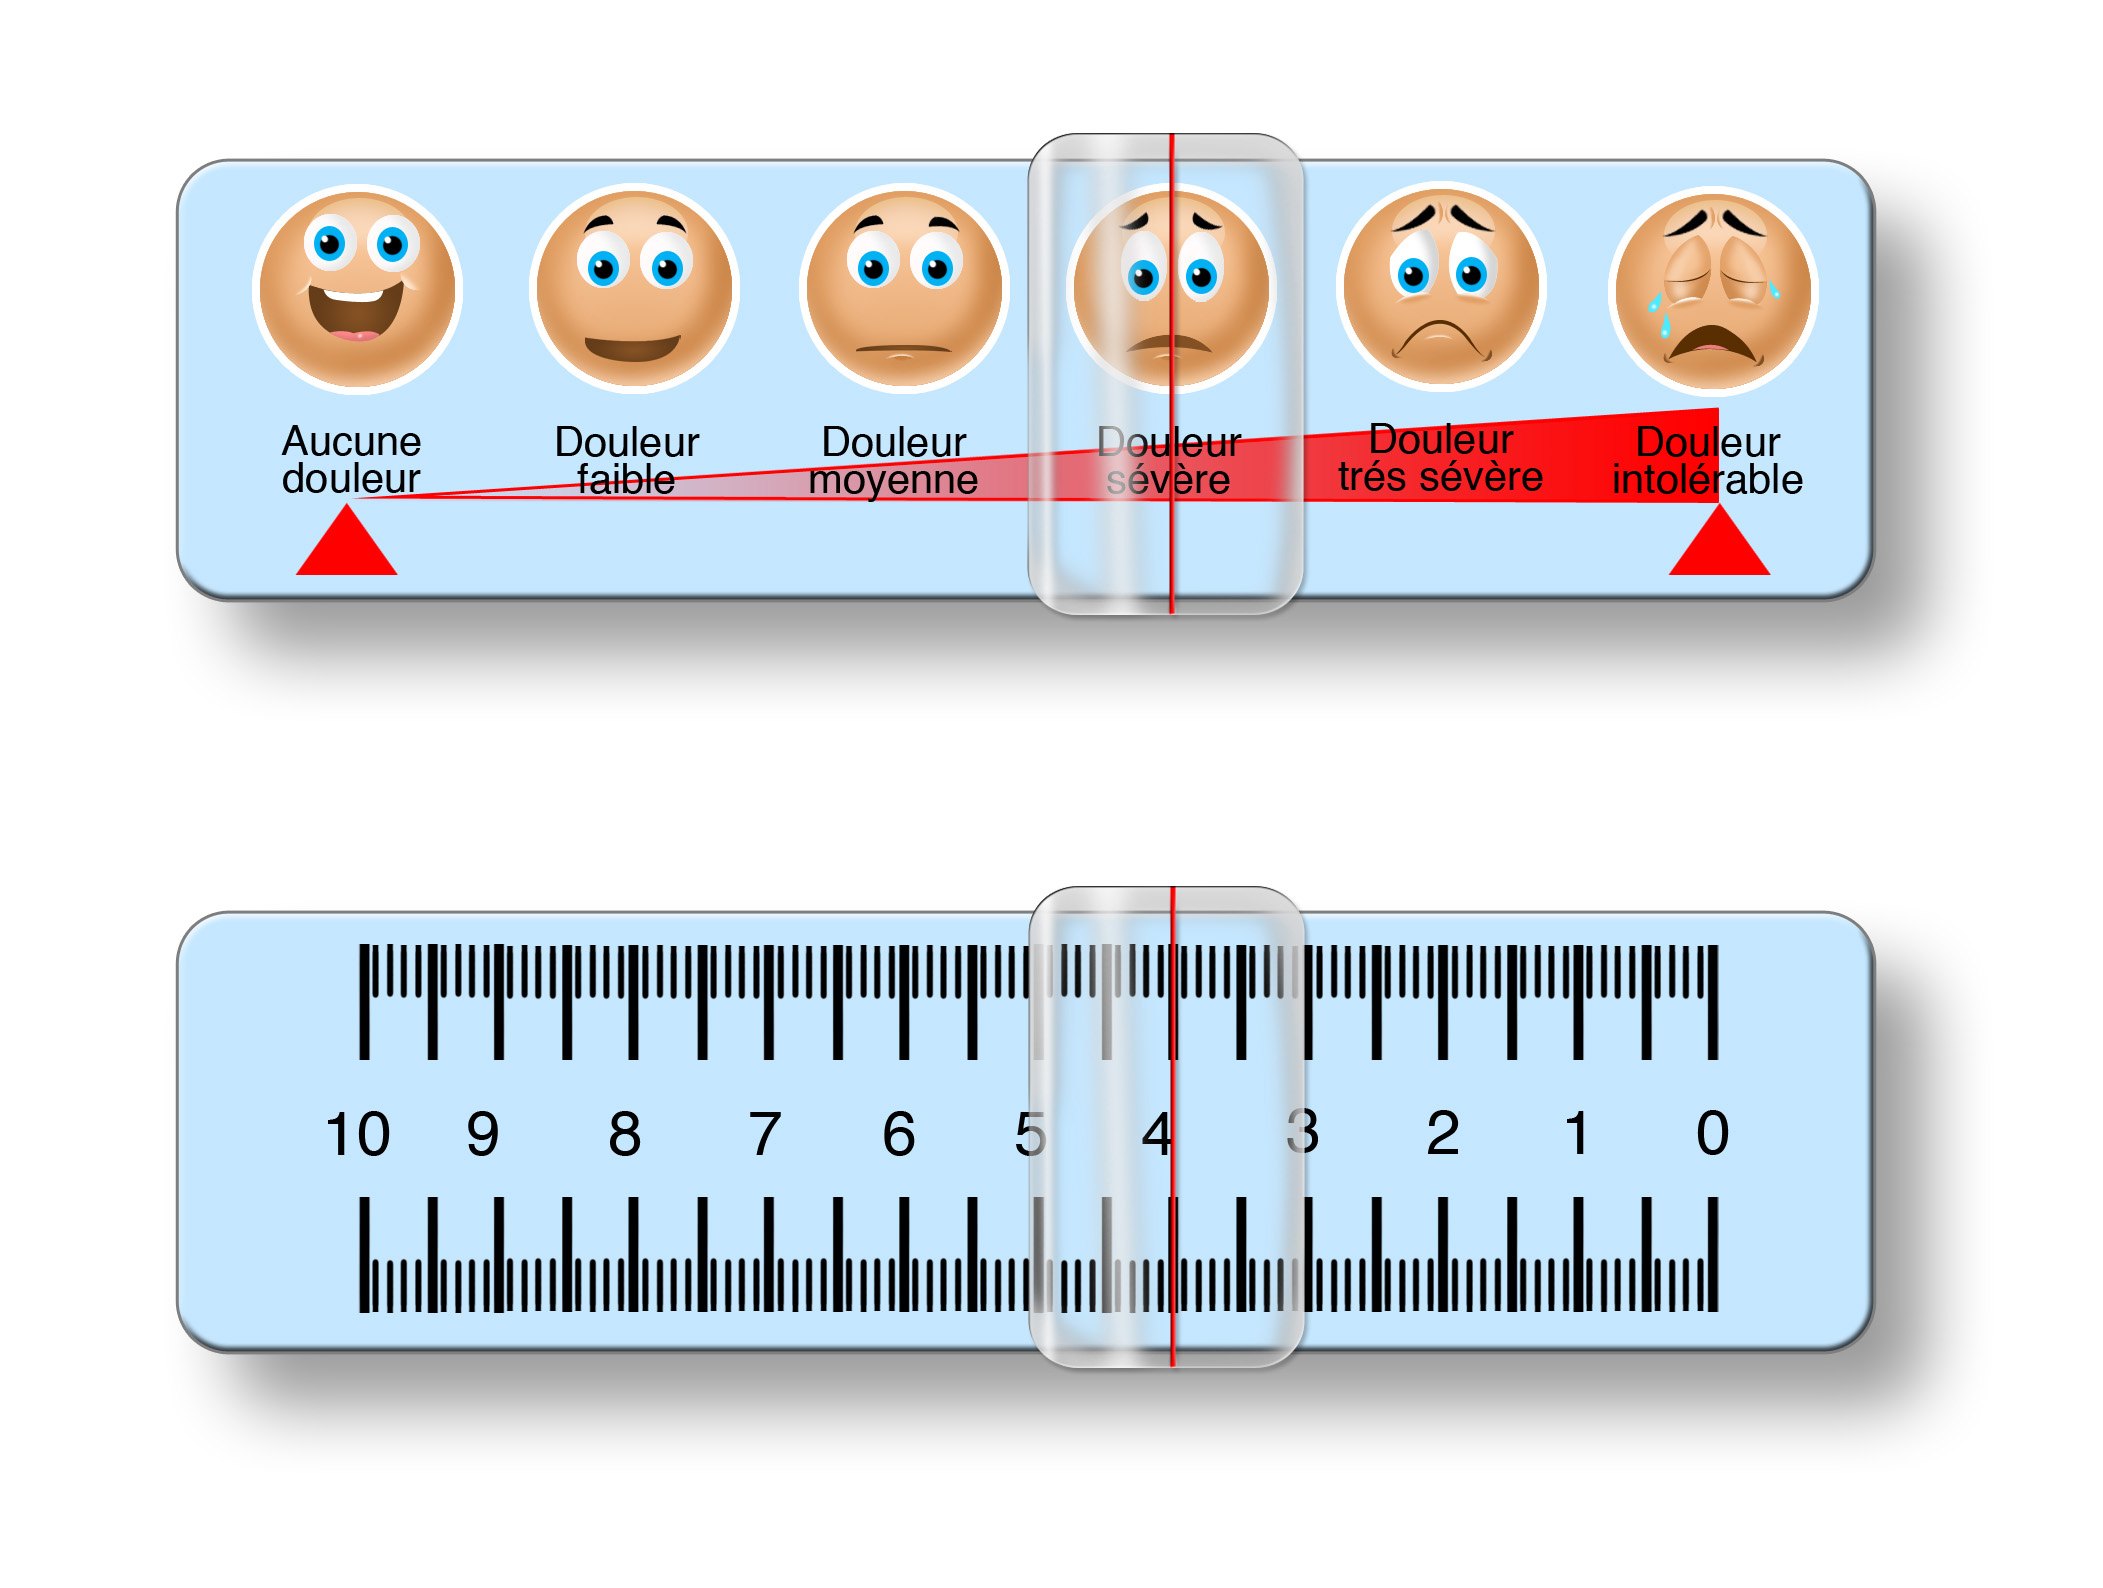
\includegraphics[height=.8\textheight]{fig/echelle-douleur.jpg}
\end{center}
\end{frame}

\begin{frame}{Organisation de la mémoire d'un ordinateur}
\begin{itemize}
\item Elle peut être vue comme un tableau d'octets avec :
\begin{itemize}
\item en \textit{indice} : le numéro de la case mémoire (commençant à 0) appelée l'\textbf{adresse}
\item en \textit{valeur} : la valeur de l'octet de la case mémoire référencée par l'indice
\end{itemize}
\end{itemize}
\begin{center}
\begin{tabular}{|l|l|}
\hline \textbf{adresse} & \textbf{valeur} \\
\hline 0 & ? \\
1 & ? \\
... & \\
234532 & 244 \\
... & \\
$n-1$ & \\
\hline
\end{tabular}
\end{center}
\end{frame}

\begin{frame}[fragile]
\frametitle{Déclaration d'une variable locale}
\begin{itemize}
\item Que se passe-t-il lorsqu'on déclare une variable ?
\begin{lstlisting}
char x = 'a';
\end{lstlisting}
\item Le système réserve une place en mémoire qui contient la valeur de \texttt{x}
\begin{itemize}
\item Il trouve une place libre (par exemple 22222)
\item dans la case associée, il stocke la valeur de la variable (ici \texttt{'a'})
\end{itemize}
\end{itemize}
\begin{center}
\begin{tabular}{|l|l|}
\hline \textbf{adresse} & \textbf{valeur} \\
\hline 0 & ? \\
1 & ? \\
... & \\
22222 & \texttt{'a'} \\
... & \\
$n-1$ & \\
\hline
\end{tabular}
\end{center}
\end{frame}

\begin{frame}[fragile]
\frametitle{Adresse d'une variable}
\begin{itemize}
\item En C(++), on peut demander l'adresse d'une variable : il suffit de préfixer son nom avec \&
%\begin{lstlisting}
%&x
%\end{lstlisting}
\item \texttt{\&x} représente l'adresse de \texttt{x}, c'est-à-dire 22222
\item Les adresses sont de simples entiers, mais C(++) permet de les typer par sécurité
\item Pointeur sur le type \textit{t} = adresse d'une variable de type \textit{t}
\item Exemples
\begin{itemize}
\item pointeur sur un entier : \texttt{int *}
\item pointeur sur un caractère : \texttt{char *}
\end{itemize}
\end{itemize}
\begin{lstlisting}
char *ptrX;
ptrX = &x;
\end{lstlisting}
\end{frame}

\begin{frame}[fragile]
\frametitle{Déréférencement}
\begin{itemize}
\item Déréférencement : accéder à la case mémoire \textit{pointée} par une adresse \texttt{t}
\item notation : \texttt{*t}
\end{itemize}
\begin{lstlisting}
cout << x << endl;
cout << *ptrX << endl;
\end{lstlisting}
\pause\begin{exampleblock}{Jouons un peu : qu'affiche ce bout de code ?}
\begin{lstlisting}
int a = 123;
int *x = &a;
*x = 342;
cout << a << endl;
cout << *x << endl;
\end{lstlisting}
\end{exampleblock}
\pause\begin{block}{Réponse}
342 \\
342
\end{block}
\end{frame}


% application des pointeurs

\begin{frame}[fragile]
\frametitle{Application des pointeurs : modifications des paramètres d'une fonction}
\begin{itemize}
\item Exemple d'une fonction qu'on ne sait pas écrire sans pointeurs : échange de deux variables
\item Passage par adresse (par opposition au passage par valeur)
\end{itemize}
\begin{lstlisting}
void echange(int *a,int *b) {
  int c = *a;
  *a = *b;
  *b = c;
}

// appel
int x = 124;
int y = 653;
echange(&x,&y);
cout << x << "," << y << endl;
\end{lstlisting}

\end{frame}

\begin{frame}[fragile]
\frametitle{Application des pointeurs : fonction retournant plusieurs valeurs}
\begin{lstlisting}
void sommediff(int a,int b,int *somme,int *diff) {
  *somme = a+b;
  *diff = a-b;
}

// appel
int s,d;
sommediff(23,18,&s,&d);
cout << s << "," << d << endl;
\end{lstlisting}

\end{frame}

% passage par adresse
\begin{frame}{Passage par adresse}
\begin{itemize}
\item Passer un paramètre à une fonction consiste à ce que la fonction reçoive \textbf{une copie} du paramètre dans une variable (qui porte le même nom ou pas)
\item Conséquence : si on modifie la copie, l'original n'est pas affecté
\item Que se passe-t-il si le paramètre est un pointeur ?
\begin{itemize}
\item Une \textbf{copie du pointeur} est fournie à la fonction appelée
\item La valeur de la copie (l'adresse) pointée ne sera jamais modifiée
\item Mais le contenu peut l'être par déréférencement
\end{itemize}
\end{itemize}
\end{frame}

\begin{frame}[fragile]
\frametitle{Rappel : pointeurs et structures de données}
\begin{itemize}
\item Si on a un type $A$ défini par \texttt{struct} ou \texttt{class}, un pointeur se définit par \texttt{A* ptr}
\item Comment accéder à un attribut \texttt{attr} de $A$ associé à \texttt{ptr} ?
\begin{itemize}
\item Logiquement : \texttt{(*ptr).attr} (attention aux priorités)
\item Raccourci : C(++) fournit une notation plus simple : \texttt{ptr->attr}
\end{itemize}
\item Attention : si le pointeur n'est pas initialisé, le déréférencement est une activité risquée...
\end{itemize}
\begin{exampleblock}{Exemple}
\begin{lstlisting}[language=C++]
int x;
int *y;
int z=*y;
\end{lstlisting}
\end{exampleblock}
\end{frame}

\subsubsection{Allocation dynamique de mémoire}

\begin{frame}[fragile]
\frametitle{Allocation mémoire en C}
\begin{itemize}
\item Allocation dynamique : réserver de la mémoire pendant l'exécution du programme
\item Réservation de mémoire avec \texttt{malloc}
\begin{lstlisting}
#include <stdio.h>
...
int *a = malloc(sizeof(int)));
struct machin *b = malloc(sizeof(struct machin));
// tableau
int *c = malloc(10*sizeof(int));
c[0] = 1; c[1] = 3;
\end{lstlisting}
\item l'opérateur \texttt{sizeof()} permet de connaître la taille d'une structure de données
\item Libération avec \texttt{free}
\begin{lstlisting}
free(a);
free(b);
free(c);
\end{lstlisting}
\end{itemize}
\end{frame}

\begin{frame}{Remarques}
\begin{itemize}
\item Penser à bien utiliser \texttt{sizeof()}, la taille des structures dépend de l'environnement d'exécution
\item De fait \texttt{malloc} et \texttt{free} ne sont pas typés et fonctionnent avec des \texttt{void *}
\item Ce sont de simples fonctions standard, on peut en utiliser d'autres (API Win32 par exemple)
\item Paradigme de gestion explicite de la mémoire : libérer tout ce qu'on alloue, par opposition au système de \textit{garbage collecting} à la Java
\item Mémoire pas initialisée + opérateurs pas typés + gestion explicite de la mémoire + accès tableaux pas vérifiés = une proportion significative de plantage des programmes C
\end{itemize}
\end{frame}

\begin{frame}[fragile]
\frametitle{Allocation mémoire en C++}
\begin{itemize}
\item Cela ne va pas résoudre tous les problèmes !
\item Réservation de mémoire avec l'opérateur \texttt{new}
\begin{lstlisting}
int *a = new int;
machin *b = new machin;
int *c = new int[10];
\end{lstlisting}
\item Plus besoin de spécifier la taille, plus de problème de type
\item Libération de la mémoire
\begin{lstlisting}
delete a;
delete b;
delete[] c;
\end{lstlisting}
\item Attention, il y a un piège !
\end{itemize}
\end{frame}

\begin{frame}[fragile]
\frametitle{Tableaux et pointeurs}
\begin{itemize}
\item Notion d'arithmétique de pointeurs...
\begin{lstlisting}
void f1() {
    int *a = new int[10];
    int *b = a;
    int i=0;
    while (i<9) {
        *b = i;
        b++; i++;
    }
    *b = i;

    for (int j=0 ; j<10 ; j++) {
        cout << "a[" << j << "] = " << a[j] << endl;
    }

    delete[] a;
}
\end{lstlisting}
\item On peut appliquer additions et soustractions aux pointeurs
\begin{itemize}
\item l'unité est la taille du type de l'élément pointé
\item utile pour parcourir vite des tableaux, mais dangereux à souhait
\item aucune vérification de validité n'est effectuée...
\end{itemize}
\end{itemize}
\end{frame}
% arithmetique de pointeurs

% effets de bord
\begin{frame}{Exercice}
\begin{itemize}
\item Écrire un petit bout de code qui parcourt un tableau avec des pointeurs en dépassant la taille du tableau
\item Que se passe-t-il
\begin{itemize}
\item s'il n'y a rien d'autre dans la fonction ?
\item si juste après la déclaration du tableau, d'autres variables sont déclarées ?
\end{itemize}
\item La réponse dépend du compilateur...
\end{itemize}
\end{frame}
% le pointeur void * et les conversions de type

\begin{frame}[fragile]
\frametitle{Le pointeur void *}
\begin{itemize}
\item On a vu que certaines fonctions retournaient un type \texttt{void *}
\item \textit{void} en anglais signifie "rien, nul", voir fonction qui ne retourne rien
\item Que signifie alors \texttt{void *} ? juste une adresse en mémoire, non typée
\item Attention : c'est un format d'échange de tout vers n'importe quoi...
\begin{lstlisting}
    int a[10];
    float *b;

    b = (float *)((void *) a);
\end{lstlisting}
\end{itemize}
\end{frame}
% lien entre pointeurs et tableaux

% un bout sur les smart pointers ?
